\documentclass{article}

\usepackage{fancyhdr}
\usepackage{extramarks}
\usepackage{amsmath}
\usepackage{amsthm}
\usepackage{amsfonts}
\usepackage{tikz}
\usetikzlibrary{3d}
\usepackage[plain]{algorithm}
\usepackage{algpseudocode} 
\usepackage{braket}
\usepackage{enumerate}
\usepackage{paralist}

%
% Basic Document Settings
%

\topmargin=-0.45in
\evensidemargin=0in
\oddsidemargin=0in
\textwidth=6.5in
\textheight=9.0in
\headsep=0.25in

\linespread{1.1}

\pagestyle{fancy}
\lhead{Habib University}
\chead{\hmwkClass, \hmwkTitle}
\rhead{\firstxmark}
\lfoot{\lastxmark}
\cfoot{\thepage}

\renewcommand\headrulewidth{0.4pt}
\renewcommand\footrulewidth{0.4pt}

\setlength\parindent{0pt}

%
% Create Problem Sections
%

\newcommand{\enterProblemHeader}[1]{
	\nobreak\extramarks{}{Problem \arabic{#1} continued on next page\ldots}\nobreak{}
	\nobreak\extramarks{Problem \arabic{#1} (continued)}{Problem \arabic{#1} continued on next page\ldots}\nobreak{}
}

\newcommand{\exitProblemHeader}[1]{
	\nobreak\extramarks{Problem \arabic{#1} (continued)}{Problem \arabic{#1} continued on next page\ldots}\nobreak{}
	\stepcounter{#1}
	\nobreak\extramarks{Problem \arabic{#1}}{}\nobreak{}
}

\setcounter{secnumdepth}{0}
\newcounter{partCounter}
\newcounter{homeworkProblemCounter}
\setcounter{homeworkProblemCounter}{1}
\nobreak\extramarks{Problem \arabic{homeworkProblemCounter}}{}\nobreak{}

%
% Homework Problem Environment
%
% This environment takes an optional argument. When given, it will adjust the
% problem counter. This is useful for when the problems given for your
% assignment aren't sequential. See the last 3 problems of this template for an
% example.
%
\newenvironment{homeworkProblem}[1][-1]{
	\ifnum#1>0
	\setcounter{homeworkProblemCounter}{#1}
	\fi
	\section{Problem \arabic{homeworkProblemCounter}}
	\setcounter{partCounter}{1}
	\enterProblemHeader{homeworkProblemCounter}
}{
	\exitProblemHeader{homeworkProblemCounter}
}

%
% Homework Details
%   - Title
%   - Due date
%   - Class
%   - Section/Time
%   - Instructor
%   - Author
%

\newcommand{\hmwkTitle}{Homework\ \#1}
\newcommand{\hmwkDueDate}{September 27, 2026, 11.59pm}
\newcommand{\hmwkClass}{CS/PHYS  314/300: Quantum Computing}
\newcommand{\hmwkClassInstructor}{Dr. Faisal Alvi}
\newcommand{\hmwkAuthorName}{\textbf{Sameez Sarfaraz Sajwani, ss09212} \and \textbf{Hassan Akhter, ha10609}}

%
% Title Page
%

\title{
	\vspace{2in}
	\textmd{\textbf{\hmwkClass:\\ \hmwkTitle}}\\
	\normalsize\vspace{0.1in}\small{\hmwkClassInstructor}\\
	\normalsize\vspace{0.1in}\small{Due\ on\ \hmwkDueDate}\\
	\vspace{3in}
}

\author{\hmwkAuthorName}
\date{}

\renewcommand{\part}[1]{\textbf{\large Part \Alph{partCounter}}\stepcounter{partCounter}\\}

%
% Various Helper Commands
%

% Useful for algorithms
\newcommand{\alg}[1]{\textsc{\bfseries \footnotesize #1}}

% For derivatives
\newcommand{\deriv}[1]{\frac{\mathrm{d}}{\mathrm{d}x} (#1)}

% For partial derivatives
\newcommand{\pderiv}[2]{\frac{\partial}{\partial #1} (#2)}

% Integral dx
\newcommand{\dx}{\mathrm{d}x}

% Alias for the Solution section header
\newcommand{\solution}{\textbf{\large Solution}}

% Probability commands: Expectation, Variance, Covariance, Bias
\newcommand{\E}{\mathrm{E}}
\newcommand{\Var}{\mathrm{Var}}
\newcommand{\Cov}{\mathrm{Cov}}
\newcommand{\Bias}{\mathrm{Bias}}

\begin{document}

\maketitle

\pagebreak

\begin{homeworkProblem}
	(10 points) Given a qubit $\ket{\psi} = \alpha \ket{0} + \beta \ket{1}$, and an operator denoted by a matrix $U$, prove that

	\begin{enumerate}[(a)]
		\item (4 points) if $U$ is unitary, then $U$ preserves the norm of the qubit after application, i.e., $|| \ket{\psi} || = ||\; U\ket{\psi} ||$.
		\item (3 points) the rows of $U$ are orthonormal to each other.
		\item (3 points) the columns of $U$ are orthonormal to each other.
	\end{enumerate}

	\textbf{Solution}
	\begin{itemize}
		\item[(a)] $\|\ket{\psi} = U\ket{\psi}\|$
		      we take the square norm of the quantum state after applying the Unitary operation \\
		      $\| U\ket{\psi} \|^2 = (U\ket{\psi})^\dagger (U\ket{\psi})$ \\
		      $(U\ket{\psi})^\dagger = \bra{\psi}U^\dagger $ \\
		      Therefore, $\braket{\psi | U^\dagger U | \psi} \overset{U^\dagger U = I} = \braket{\psi | I | \psi} = \braket{\psi | \psi} = \| \ket{\psi}^2 \|$ \\
		      $$ \|U\ket{\psi}\|^2 = \| \ket{\psi} \|^2$$
		      $$ \|U\ket{\psi}\| = \| \ket{\psi} \|$$
		      Thus we have proven that unitary operations on a qubit do not affect its total probability, i.e sum of the new probabilites will always equal 1.

		\item[(b)] rows are orthonormal if: \\
		      Norm of the row is 1. \\
		      Inner Product between rows is 0. \\
		      For a 2x2 matrix, $U U^\dagger = \begin{pmatrix} a & b  \\ c & d  \end{pmatrix} \begin{pmatrix} a^* & c^*  \\ b^* & d^*  \end{pmatrix} = \begin{pmatrix} 1 & 0 \\ 0 & 1 \end{pmatrix} = I$ \\
		      Such that, $\| r1 \| = \| r2 \| = 1$, and $\langle r1,r2 \rangle = 0$. Where $\| r1 \|^2 = |a|^2 + |b|^2$, $\| r2 \|^2 = |c|^2 + |d|^2$, and $\langle r1,r2 \rangle$ is the inner product between r1,r2: $ac^* + bd^*$, $ca^* + db^*$. \\
		      If the resulting matrix of any such arbitary matrix U matches the Identity Matrix, we have proven that U's rows are orthonormal to each other as $UU^\dagger = I$, this logic can be extended to n dimensions.
		      .

		\item[(c)] Columns are orthonormal if: \\
		      Norm of the columns is 1. \\
		      Inner Product between columns is 0. \\
		      For a 2x2 matrix, $U^\dagger U = \begin{pmatrix} a^* & c^*  \\ b^* & d^*  \end{pmatrix} \begin{pmatrix} a & b  \\ c & d  \end{pmatrix} = \begin{pmatrix} 1 & 0 \\ 0 & 1 \end{pmatrix} = I$ \\
		      Such that, $\| c1 \| = \| c2 \| = 1$, and $\langle c1,c2 \rangle = 0$. Where $\| c1 \|^2 = |a|^2 + |c|^2$, $\| c2 \|^2 = |b|^2 + |d|^2$, and $\langle c1,c2 \rangle$ is the inner product between c1,c2: $a^*b + c^*d$, $b^*a + d^*c$.
		      If the resulting matrix of any such arbitary matrix U matches the identity Matrix, we have proven that U's columns are orthonormal to each other as $U^\dagger U = I$, this logic can be extended to n dimensions.
	\end{itemize}
\end{homeworkProblem}
\newpage

\begin{homeworkProblem}
	(10 points) Consider a Bloch Sphere representation of a qubit $\ket{\psi} = \cos(\theta/2)\ket{0} + e^{(i\phi)} \sin(\theta/2)\ket{1}$ as shown here.

	\begin{figure} [H]
		\centering
		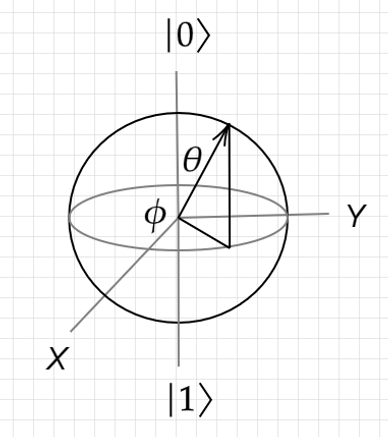
\includegraphics[scale = 0.7]{Bloch-Sphere.png}
		\caption{Bloch sphere representation of an arbitrary qubit state $\ket{\psi} = \cos(\theta/2)\ket{0} + e^{(i\phi)} \sin(\theta/2)\ket{1}$}
	\end{figure}
	On the Bloch Sphere, plot the following qubits (show a plot similar to a diagram above):
	\begin{enumerate}[(a)]
		\item (2 points) \[\frac{\sqrt{3}}{2}|0\rangle + \frac{i}{2}|1\rangle\]
		\item (3 points) \[ \frac{1-i}{2}|0\rangle + \frac{1+i}{2}|1\rangle\]
	\end{enumerate}
	Next, consider the following operations:
	\[
		(i) \;\;	R(\theta_1) = \begin{bmatrix}
			\cos(\theta_1) & -\sin(\theta_1) \\
			\sin(\theta_1) & \cos(\theta_1)
		\end{bmatrix},
		(ii) \;\;	S(\phi_2) = \begin{bmatrix}
			e^{-i\phi_2} & 0           \\
			0            & e^{i\phi_2}
		\end{bmatrix}\]
	Given an arbitrary qubit on the $X$-$Z$ plane (i.e.) its amplitudes have no imaginary component, \\
	\begin{enumerate}
		\setcounter{enumi}{2} % start from C (A=0, B=1, C=2)
		\renewcommand{\labelenumi}{(\alph{enumi})}
		\item (2 points) what is the effect of applying $R(\theta_1)$ to it? In particular state the effect when $\theta_1 = \pi/2$?\\

		\item (3 points) what is the effect of applying $S(\phi_2)$ to it? In particular state the effect when $\phi_2 = \pi/2$?\\
	\end{enumerate}
	\textbf{Solution}
	\begin{itemize}
		\item[(a)] $\frac{\sqrt{3}}{2}\ket{0} + \frac{i}{2}\ket{1}$ \\
		      $\cos(\frac{\theta}{2})\ket{0} + e^{-i\frac{\pi}{2}}\frac{1}{2}\sin(\frac{\theta}{2}\ket{1}$ \\
		      $\theta = 2\cos^-1(\frac{\sqrt{3}}{2}) =$ 60 degrees, 1.047rad, $\phi = \frac{\pi}{2} = 90$ degrees \\
		\item[(b)] $\frac{1-i}{2}\ket{0} + \frac{1+i}{2}\ket{1}$ \\
		      $e^{-i\frac{\pi}{4}} \left( \frac{1}{\sqrt{2}}\ket{0} + e^{i\frac{\pi}{2}}\frac{1}{\sqrt{2}}\ket{1} \right)$ \\
		      $\cos(\frac{\theta}{2})\ket{0} + e^{i\frac{\pi}{2}}\sin(\frac{\theta}{2})\ket{1}$ \\
		      $\theta = 2\cos^{-1}(\frac{1}{\sqrt{2}}) =$ 90 degrees, 1.571rad, $\phi = \frac{\pi}{2} =$ 90 degrees \\
	\end{itemize}

	\begin{figure}
		\centering
		\begin{minipage}{0.45\textwidth}
			\centering
			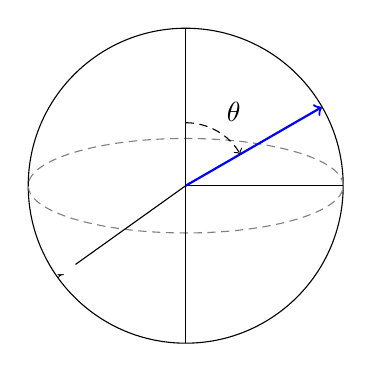
\begin{tikzpicture}[scale=2]
				% Sphere boundary
				\draw (0,0) circle (1cm);
				% Equator
				\draw[gray, densely dashed] (0,0) ellipse (1cm and 0.3cm);
				% Back half of equator
				\clip (0,0) circle (1cm);

				% Axes
				\draw[-] (0,0) -- (0,1.3) node[above] {$|0\rangle$};
				\draw[-] (0,0) -- (0,-1.3) node[below] {$|1\rangle$};
				\draw[-] (0,0) -- (-0.7,-0.5) node[below left] {$X$};
				\draw[-] (0,0) -- (1.3,0) node[right] {$Y$};

				% Vector (a): theta = 60 degrees, phi = 90 degrees (on Y-Z plane)
				% TikZ standard angles: right is 0, up is 90. 
				% So 60 deg from Z-axis is x=sin(60), y=cos(60)
				\draw[->, thick, blue] (0,0) -- ({sin(60)}, {cos(60)}) node[above right] {$|\psi_a\rangle$};

				% Theta Angle indicator
				\draw[->, densely dashed] (0,0.4) arc (90:30:0.4) node[midway, above right] {$\theta$};
			\end{tikzpicture} \\
			(a): $\theta = \pi/3, \phi = \pi/2$
		\end{minipage}\hfill
		% State (b)
		\begin{minipage}{0.45\textwidth}
			\centering
			\begin{tikzpicture}[scale=2]
				% Sphere boundary
				\draw (0,0) circle (1cm);
				% Equator$$ S(\phi_2)\ket{\psi} = \begin{pmatrix} e^{-i\phi_2} & 0 \\ 0 & e^{i\phi_2} \end{pmatrix} \begin{pmatrix} a \\ b \end{pmatrix} = \begin{pmatrix} a e^{-i\phi_2} \\ b e^{i\phi_2} \end{pmatrix} $$
				Factoring out a global phase of $e^{-i\phi_2}$, the state becomes $a\ket{0} + b e^{i(2\phi_2)}\ket{1}$. This operation rotates the qubit around the Z-axis by an angle of $2\phi_2$. For most values of $\phi_2$, this introduces a complex phase, pulling the qubit off the X-Z plane and into the Y-dimension.
				\draw[gray, densely dashed] (0,0) ellipse (1cm and 0.3cm);

				% Axes
				\draw[-] (0,0) -- (0,1.3) node[above] {$|0\rangle$};
				\draw[-] (0,0) -- (0,-1.3) node[below] {$|1\rangle$};
				\draw[-] (0,0) -- (-0.7,-0.5) node[below left] {$X$};
				\draw[-] (0,0) -- (1.3,0) node[right] {$Y$};

				% Vector (b): theta = 90 degrees, phi = 90 degrees (+Y axis)
				\draw[->, thick, red] (0,0) -- (1,0) node[above right] {$|\psi_b\rangle$};

				% Theta Angle indicator
				\draw[->, densely dashed] (0,0.4) arc (90:0:0.4) node[midway, above right] {$\theta$};
			\end{tikzpicture} \\
			(b): $\theta = \pi/2, \phi = \pi/2$
		\end{minipage}
	\end{figure}
	\begin{itemize}
		\item[(c)]
		      The arbitrary qubit on the X-Z plane can be defined as: $\ket{\phi} = \alpha\ket{0} + \beta\ket{1} \qquad \alpha,\beta \in \mathbb{R}.$ \\
		      Therefore the qubit doesn't consist of any imaginary component.
		      $$R(\theta_1)\ket{\psi} = \begin{pmatrix} \cos(\theta_1) & -\sin(\theta_1) \\ \sin(\theta_1) & \cos(\theta_1) \end{pmatrix} \begin{pmatrix} \alpha \\ \beta \end{pmatrix} = \begin{pmatrix} \alpha\cos(\theta_1) - \beta\sin(\theta_1) \\ \alpha\sin(\theta_1) + \beta\cos(\theta_1) \end{pmatrix} $$
		      As the all componenets are real, the resulting transforamtion rotates the qubit within the X-Z plane, When $\theta_1 = \pi/2$, the qubit is rotated by 90 degrees around the y-axis (in the X-Z plane.) \\
		      the 90 degrees rotation transforms the qubit to $\ket{\psi} = -\beta\ket{0} + \alpha\ket{1}$.
		\item[(d)]
		      The arbitrary qubit as defined in the question above, when applied.
		      $$S(\phi_2)\ket{\psi} = \begin{pmatrix} e^{-i\phi_2} & 0 \\ 0 & e^{i\phi_2} \end{pmatrix} \begin{pmatrix} \alpha \\ \beta \end{pmatrix} = \begin{pmatrix} \alpha e^{-i\phi_2} \\ \beta e^{i\phi_2} \end{pmatrix} $$
		      Factoring out a global phase of $e^{-i\phi_2}$, the state becomes $\alpha\ket{0} + \beta e^{i(2\phi_2)}\ket{1}$. This operation rotates the qubit around the Z-axis by an angle of $2\phi_2$ introducing a complex phase in the Y-axis.
	\end{itemize}
\end{homeworkProblem}
\newpage

\begin{homeworkProblem}
	(10 points) So far we have studied qubits defined using two basis states: $\ket{0}$ and $\ket{1}$. We have also seen two related states: the $\ket{+}$ state and the $\ket{-}$ state. Answer the following questions with reasons:

	\begin{enumerate}[(a)]
		\item(2 points) Do the $\ket{+}$ state and the $\ket{-}$ state form a pair of orthonormal states?
		\item (2 points) Can the $\ket{+}$ state and the $\ket{-}$ state be used as the basis states?
		\item If the answer to the both (a) and (b) is Yes, express the following qubits as a linear combination of the $\ket{+}$ state and the $\ket{-}$ state:

		      (i) (2 points) $\ket{0}$,

		      (ii) (2 points) $\ket{1}$,

		      (iii) (2 points) an arbitrary qubit: $\ket{\psi} = \alpha \ket{0} + \beta \ket{1}$.

	\end{enumerate}

	\solution

	\begin{enumerate} [(a)]
		\item for $\ket{0}, \ket{1}$ to be a valid pair of orthonormal states, we need them to be orthogonal to each other (i.e. their inner product equals 0) and normal (they both must have unit norm). \\
		      \textbf{Representation:} \\
		      $\ket{+} = \frac{1}{\sqrt{2}} (\ket{0} + \ket{1}) = \begin{pmatrix}\frac{1}{\sqrt{2}} \\ \frac{1}{\sqrt{2}}\end{pmatrix}$ \\


		      $\ket{-} = \frac{1}{\sqrt{2}} (\ket{0} - \ket{1}) = \begin{pmatrix}\frac{1}{\sqrt{2}} \\ \frac{-1}{\sqrt{2}}\end{pmatrix}$ \\

		      \textbf{Orthogonality:} \\
		      $\bra{+}\ket{-} = \begin{pmatrix} \frac{1}{\sqrt{2}} & \frac{1}{\sqrt{2}} \end{pmatrix} \begin{pmatrix} \frac{1}{\sqrt{2}} \\ \frac{-1}{\sqrt{2}} \end{pmatrix} = (\frac{1}{\sqrt{2}} \times \frac{1}{\sqrt{2}}) + (\frac{1}{\sqrt{2}} \times \frac{-1}{\sqrt{2}}) = \frac{1}{2} + \frac{-1}{2} = \frac{1}{2} - \frac{1}{2} = 0$ \\

		      $\bra{-}\ket{+} = \begin{pmatrix} \frac{1}{\sqrt{2}} & \frac{-1}{\sqrt{2}} \end{pmatrix} \begin{pmatrix} \frac{1}{\sqrt{2}} \\ \frac{1}{\sqrt{2}} \end{pmatrix} = (\frac{-1}{\sqrt{2}} \times \frac{1}{\sqrt{2}}) + (\frac{1}{\sqrt{2}} \times \frac{1}{\sqrt{2}}) = \frac{-1}{2} + \frac{1}{2} = \frac{1}{2} - \frac{1}{2} = 0$ \\

		      Therefore, $\ket{+}, \ket{-}$ are orthogonal \\

		      \textbf{Normality:} \\
		      $\ket{+} = \alpha \ket{0} + \beta \ket{1}$ where $\alpha = \beta = \frac{1}{\sqrt{2}}$. It's norm is $\sqrt{\alpha^2 + \beta^2} = \sqrt{(\frac{1}{\sqrt{2}})^2 + (\frac{1}{\sqrt{2}})^2} = \sqrt{\frac{1}{2} + \frac{1}{2}} = \sqrt{1} = 1$ \\
		      $\ket{-} = \alpha \ket{0} + \beta \ket{1}$ where $\alpha = \frac{1}{\sqrt{2}}, \beta \frac{-1}{\sqrt{2}}$. It's norm is $\sqrt{\alpha^2 + \beta^2} = \sqrt{(\frac{1}{\sqrt{2}})^2 + (\frac{-1}{\sqrt{2}})^2} = \sqrt{\frac{1}{2} + \frac{1}{2}} = \sqrt{1} = 1$ \\

		      Therefore $\ket{+}, \ket{-}$ can form an orthonormal pair of basis quantum states.

		\item Yes. For any pair of qubits $\ket{\phi_1}, \ket{\phi_2}$ to act as a basis, they must be orthonormal to each other (orthogonal to each other and have unit norm). Since $\ket{+}, \ket{-}$ satisfy the criteria, they can also act as a valid pair of basis states to represent a qubit.

		\item We can represent qubits in terms of $\ket{+}, \ket{-}$ as follows:
		      \begin{enumerate}[(i)]
			      \item $\ket{+} + \ket{-} = (\frac{1}{\sqrt{2}} \ket{0} + \frac{1}{\sqrt{2}} \ket{1}) + (\frac{1}{\sqrt{2}} \ket{0} - \frac{1}{\sqrt{2}}\ket{1}) = \frac{1}{\sqrt{2}} \ket{0} + \frac{1}{\sqrt{2}} \ket{1} + \frac{1}{\sqrt{2}} \ket{0} - \frac{1}{\sqrt{2}} \ket{1} = \frac{2}{\sqrt{2}} \ket{0}$. Therefore, $\ket{0} = \frac{\sqrt{2}}{2} (\ket{+} + \ket{-}) = \frac{1}{\sqrt{2}} (\ket{0} + \ket{1})$
			      \item $\ket{+} - \ket{-} = (\frac{1}{\sqrt{2}} \ket{0} + \frac{1}{\sqrt{2}} \ket{1}) - (\frac{1}{\sqrt{2}} \ket{0} - \frac{1}{\sqrt{2}}\ket{1}) = \frac{1}{\sqrt{2}} \ket{0} + \frac{1}{\sqrt{2}} \ket{1} - \frac{1}{\sqrt{2}} \ket{0} + \frac{1}{\sqrt{2}} \ket{1} = \frac{2}{\sqrt{2}} \ket{1}$. Therefore, $\ket{1} = \frac{\sqrt{2}}{2} (\ket{+} - \ket{-}) = \frac{1}{\sqrt{2}} (\ket{0} - \ket{1})$
			      \item using the representations above, we can represent any arbitrary qubit as follows: \\
			            $\ket{\psi} = \alpha \ket{0} + \beta \ket{1} = \alpha \times \frac{1}{\sqrt{2}} (\ket{+} + \ket{-}) + \beta \times \frac{1}{\sqrt{2}} (\ket{+} - \ket{-}) = \frac{\alpha}{\sqrt{2}} \ket{+} + \frac{\alpha}{\sqrt{2}} \ket{-} + \frac{\beta}{\sqrt{2}} \ket{+} - \frac{\beta}{\sqrt{2}} \ket{-} = \frac{\alpha + \beta}{\sqrt{2}} \ket{+} + \frac{\alpha - \beta}{\sqrt{2}} \ket{-}$
		      \end{enumerate}

	\end{enumerate}
\end{homeworkProblem}
\newpage

\begin{homeworkProblem}
	The Pauli Matrices are given by:

	\[
		X = \sigma_x = \begin{pmatrix}
			0 & 1 \\
			1 & 0
		\end{pmatrix}
		\quad
		Y = \sigma_y = \begin{pmatrix}
			0 & -i \\
			i & 0
		\end{pmatrix}
		\quad
		Z = \sigma_z = \begin{pmatrix}
			1 & 0  \\
			0 & -1
		\end{pmatrix}
	\]

	Show that the following relations hold:
	\vspace{5pt}
	\begin{compactenum}[(a)]
		\item (3 points) $HX$ = $ZH$,
		\item (3 points) $HY$ = $-YH$,
		\item (3 points) $HZ$ = $XH$.
	\end{compactenum}
	where $H$ is the Hadamard operation.
	\vspace{2pt}

	(1 point) Using these properties, show that $HXHYHZ = ZYXH$

	\vspace{5pt}

	\solution
	\begin{itemize}
		\item[(a)] we know that $H = \frac{1}{\sqrt{2}}V$, where $V = \begin{pmatrix} 1 & 1 \\ 1 & -1 \end{pmatrix}$. As we can pull any scalar factor out of a matrix multiplication, it is sufficient to show that $VX = ZV$. \\

		      $VX = \begin{pmatrix} 1 & 1 \\ 1 & -1 \end{pmatrix} \begin{pmatrix} 0 & 1 \\ 1 & 0 \end{pmatrix} = \begin{pmatrix} 1 \times 0 + 1 \times 1 & 1 \times 1 + 1 \times 0 \\ 1 \times 0 - 1 \times 1 & 1 \times 1 - 1 \times 0 \end{pmatrix} = \begin{pmatrix} 0 + 1 & 1 + 0 \\ 0 - 1 & 1 - 0 \end{pmatrix} = \begin{pmatrix} 1 & 1 \\ -1 & 1 \end{pmatrix}$ \\

		      $ZV = \begin{pmatrix} 1 & 0 \\ 0 & -1 \end{pmatrix} \begin{pmatrix} 1 & 1 \\ 1 & -1 \end{pmatrix} = \begin{pmatrix} 1 \times 1 + 0 \times 1 & 1 \times 1 + 0 \times -1 \\ 0 \times 1 - 1 \times 1 & 0 \times 1 - 1 \times (-1) \end{pmatrix} = \begin{pmatrix} 1 + 0 & 1 + 0 \\ 0 - 1 & 0 - (-1) \end{pmatrix} = \begin{pmatrix} 1 & 1 \\ -1 & 1 \end{pmatrix}$

		\item[(b)] using similar reasoning as above, we only need to show that $VY = -YV$ \\

		      $VY = \begin{pmatrix} 1 & 1 \\ 1 & -1 \end{pmatrix} \begin{pmatrix} 0 & -i \\ i & 0 \end{pmatrix} = \begin{pmatrix} 1 \times 0 + 1 \times i & 1 \times (-i) + 1 \times 0 \\ 1 \times 0 - 1 \times i & 1 \times (-i) - 1 \times 0 \end{pmatrix} =
			      \begin{pmatrix} 0 + i & -i + 0 \\ 0- i & -i - 0 \end{pmatrix} = \begin{pmatrix} i & -i \\ -i & -i \end{pmatrix}$ \\

		      $-YV = - \begin{pmatrix} 0 & -i \\ i & 0 \end{pmatrix} \begin{pmatrix} 1 & 1 \\ 1 & -1 \end{pmatrix} = - \begin{pmatrix} 0 \times 1 - i \times 1 & 0 \times 1 - i \times (-1) \\ i \times 1 + 0 \times 1 & i \times 1 + 0 \times (-1) \end{pmatrix} = - \begin{pmatrix} 0 - i & 0 + i \\ i + 0 & i + 0 \end{pmatrix} = - \begin{pmatrix} -i & i \\ i & i \end{pmatrix} = \begin{pmatrix} i & -i \\ -i & -i \end{pmatrix}$

		\item[(c)] by observation, we see that $H^T= H, X^T = X, Z^T = Z$ (they are all symmetric matrices). We can use the property of matrices $(UV)^T = V^T U^T$ to prove the property. \\
		      We have shown in part $(a)$ that $ZH = HX$. Taking transpose on both sides, \\
		      $(ZH)^T = (HX)^T$. Using the property of transpose, $H^T Z^T = X^T H^T$. \\
		      Since $H, X, Z$ are symmetric, we get $HZ = XH$

		\item[(d)] we know that $H^2 = \mathbb{I}$, where $\mathbb{I}$ is the identity matrix. \\
		      $HXHYHZ = ZHHYHZ$ using part $(a)$ \\
		      $ = ZYHZ$ using the definitions of $H, \mathbb{I}$ \\
		      $ = ZYXH$ using part $(c)$
	\end{itemize}
\end{homeworkProblem}
\newpage

\begin{homeworkProblem}
	(10 points) We have seen earlier that if we are given one of the two quantum states $\ket{+}$ and $\ket{-}$ such that it is not known whether it is a $\ket{+}$ and $\ket{-}$, we can distinguish between them \textit{perfectly} by applying a Hadamard operation followed by a measurement. \\


	Suppose we are randomly sent one of the following two states: \[ (a) \;\;
		\frac{1}{2}\ket{0} + \frac{\sqrt{3}}{2} i\ket{1}, (b) \;\; \frac{\sqrt{3}}{2}\ket{0} + \frac{1}{2}i\ket{1},
	\]

	Devise a procedure to find out which one of the two states has been sent. This procedure should perform better than a random choice with a success probability as high as possible. More specifically, given one of the two qubits, by performing your operation(s) followed by a measurement, the probability of finding out which one of the states is should be as high as possible, with the lower limit being greater than a random guess, i.e. $> 1/2$.


	\vspace{5pt}

	\textbf{Solution} \\
	The Qubit $\frac{1}{2}\ket{0} + \frac{\sqrt{3}}{2} i \ket{1}$ collpases upon its basis state as per the following probabilities. $|\alpha|^2 = 1/4 (\ket{0}), |\beta|^2 = 3/4 (\ket{1})$ \\
	Furthermore, the qubit $\frac{\sqrt{3}}{2}\ket{0} + \frac{1}{2}i\ket{1}$ collpases upon its basis state as per the following probabilities. $|\alpha|^2 = 3/4 (\ket{0}), |\beta|^2 = 1/4 (\ket{1})$ \\

	Now given that a qubit has been received, blindly guessing if its either qubit A, or B would give us the correct answer 50percent of the time. \\
	A better approach would be to measure the qubit upon reciept, if it collapses to $\ket{0}$ we can simply assume that the original qubit was B, and A if the measurement came out to be $\ket{1}$. \\
	This is because, A has a 75percent chance to collpase to 1 and B has a 75percent chance to collapse to 0, Therefore if we guess after the measurement, we are likely to guess correctly 75percent of the time. \\
\end{homeworkProblem}

\end{document}
